\subsubsection{UC3 - Inserimento richiesta in linguaggio naturale}\label{UC3}

\begin{figure}[H]
  \centering
  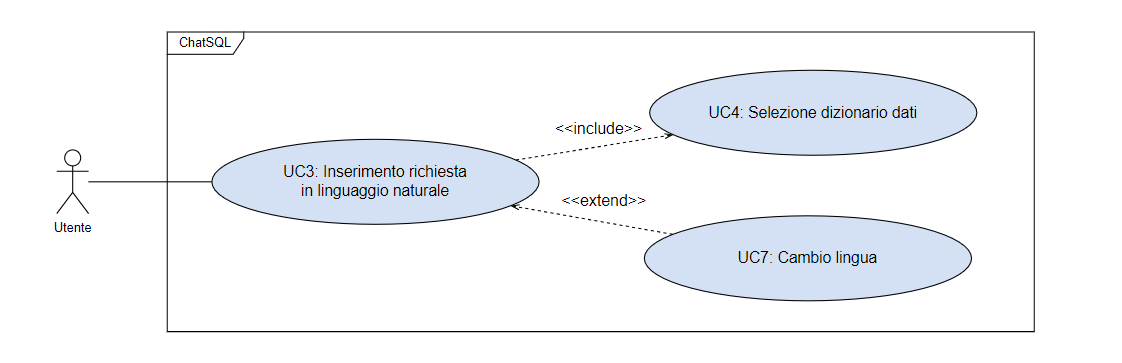
\includegraphics[width=0.90\textwidth]{assets/uc3.png}
  \caption{UC3}
\end{figure}

\paragraph*{Descrizione}
L'inserimento della richiesta in linguaggio naturale corrisponde alla digitazione, nell'apposito campo di testo, del messaggio da inviare al ChatBOT.

\paragraph*{Attori principali}
Utente

\paragraph*{Precondizioni}
\begin{itemize}
  \item L'applicazione è stata avviata con successo;
  \item L'Utente sta visualizzando correttamente la chat.
\end{itemize}

\paragraph*{Postcondizioni}
\begin{itemize}
  \item L'Utente ha scritto nell'apposito campo di testo un messaggio da inviare al ChatBOT.
\end{itemize}

\paragraph*{Trigger}
L'Utente desidera inserire una richiesta in linguaggio naturale.

\paragraph*{Scenario principale}
\begin{enumerate}
  \item L'Utente scrive una richiesta nell'apposita sezione della chat.
\end{enumerate}